\documentclass[aspectratio=169,11pt]{beamer}

% Packages
\usepackage[utf8]{inputenc}
\usepackage[T1]{fontenc}
\usepackage{lmodern}
\usepackage{microtype}
\usepackage{amsmath,amssymb}
\usepackage{booktabs}
\usepackage{graphicx}
\usepackage{tikz}
\usepackage{pgfplots}
\usepackage{xcolor}
\usepackage{ragged2e}
\usepackage{colortbl}
\usepackage{array}
\usepackage{hyperref}
\usepackage{adjustbox}

\usetikzlibrary{shapes.geometric, arrows.meta, positioning, calc, backgrounds, decorations.pathreplacing, shadows, fadings}
\pgfplotsset{compat=1.18}

% --- Color Palette: Warm Professional ---
\definecolor{DeepNavy}{HTML}{2E4057}
\definecolor{Teal}{HTML}{048A81}
\definecolor{WarmOrange}{HTML}{E85D04}
\definecolor{SoftPurple}{HTML}{9D4EDD}
\definecolor{WarmGray}{HTML}{6C757D}
\definecolor{LightGray}{HTML}{E9ECEF}
\definecolor{Cream}{HTML}{FBF8F1}
\definecolor{DeepRed}{HTML}{D62828}
\definecolor{Gold}{HTML}{D4A03A}
\definecolor{SoftWhite}{HTML}{FAFAFA}

% Beamer colors
\setbeamercolor{normal text}{fg=DeepNavy, bg=SoftWhite}
\setbeamercolor{structure}{fg=DeepNavy}
\setbeamercolor{alerted text}{fg=DeepRed}
\setbeamercolor{example text}{fg=Teal}
\setbeamercolor{frametitle}{fg=DeepNavy, bg=SoftWhite}
\setbeamercolor{title}{fg=DeepNavy}
\setbeamercolor{subtitle}{fg=WarmGray}
\setbeamercolor{block title}{bg=DeepNavy, fg=SoftWhite}
\setbeamercolor{block body}{bg=LightGray, fg=DeepNavy}
\setbeamercolor{itemize item}{fg=WarmOrange}
\setbeamercolor{itemize subitem}{fg=Gold}

% Fonts
\usefonttheme{professionalfonts}
\setbeamerfont{title}{size=\huge, series=\bfseries}
\setbeamerfont{frametitle}{size=\Large, series=\bfseries}

% Strip chrome
\setbeamertemplate{navigation symbols}{}
\setbeamertemplate{headline}{}

% Minimal footline
\setbeamertemplate{footline}{%
    \hfill
    \begin{beamercolorbox}[wd=3cm,ht=2.5ex,dp=1ex,right,rightskip=0.6cm]{page number}
        \usebeamercolor[fg]{WarmGray}\scriptsize\insertframenumber
    \end{beamercolorbox}
    \vspace{0.3cm}
}

% Bullets
\setbeamertemplate{itemize item}{\footnotesize\raisebox{0.3ex}{\tikz\fill[WarmOrange] (0,0) circle (0.45ex);}}
\setbeamertemplate{itemize subitem}{\footnotesize\raisebox{0.3ex}{\tikz\fill[Gold] (0,0) circle (0.35ex);}}

% Custom commands
\newcommand{\transitionslide}[2]{%
    {\setbeamercolor{normal text}{fg=SoftWhite,bg=DeepNavy}
    \begin{frame}[plain]\vfill\begin{center}
        {\huge\bfseries\textcolor{Gold}{#1}}\\[0.6cm]
        {\large\textcolor{LightGray}{#2}}
    \end{center}\vfill\end{frame}}
}

\begin{document}

\begin{frame}
    \title{Granular Instrumental Variables}
    \subtitle{Gabaix and Koijen (2022)}
    \author{Roy Kisluk}
    \date{}
    \titlepage
\end{frame}


%%%%%%%%%%%%%%%%%%%%%%%%%%%%%%%%%%%%%%%%%%%%%%%%%%%%%%%%%%%%%%%%%%%%%%%%%%%%%%%%
% Introduction

\begin{frame}
    \frametitle{The Law of Large Numbers fails in modern economies}

    \vspace{1cm}
    {\Large
        In a standard economy, micro-shocks cancel out at a rate of $1/\sqrt{N}$.

    }

    \vspace{1cm}
    {\Large
        In a \textbf{granular} economy, where the size distribution of firms follows a power law, a few firms are so large that their idiosyncratic luck drives aggregate volatility.
    }

\end{frame}

\begin{frame}
    \frametitle{Endogenous aggregate shocks confound the effect of large firms}

    \vspace{0.5cm}
    {\Large
        We want to estimate the elasticity of wages to labor demand.
    }

    \vspace{0.5cm}
    {\Large
        The fundamental challenge:
    }
    \vspace{0.5cm}
    \begin{center}
        \begin{adjustbox}{max width=\textwidth}
            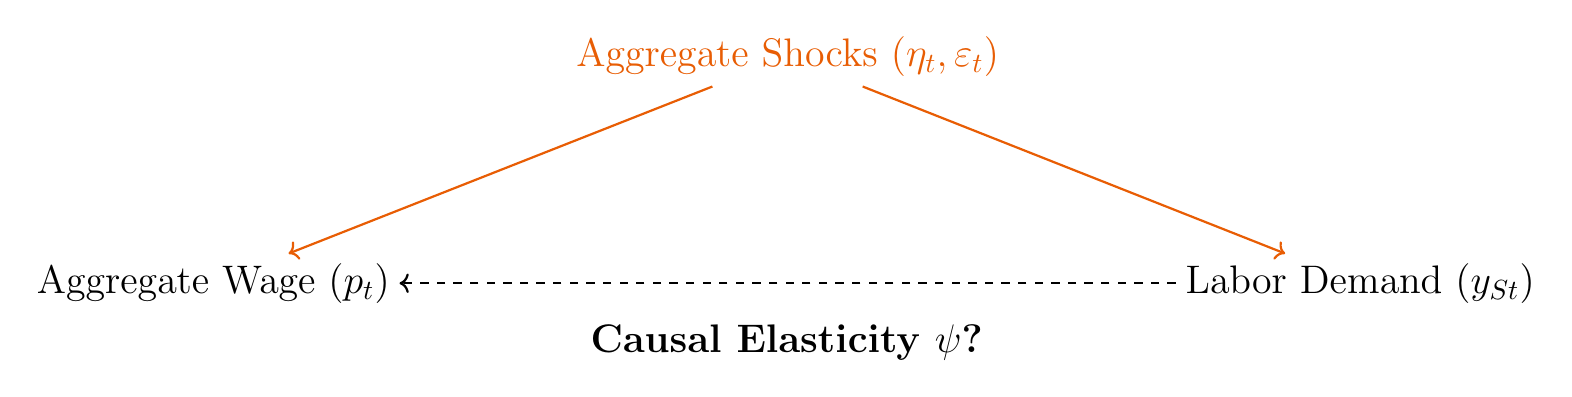
\begin{tikzpicture}[node distance=3cm, font=\Large]
                % Nodes
                \node (agg) [text=WarmOrange] {Aggregate Shocks ($\eta_t, \varepsilon_t$)};
                \node (wage) [below left=of agg] {Aggregate Wage ($p_t$)};
                \node (demand) [below right=of agg] {Labor Demand ($y_{St}$)};

                % Paths
                \draw[->, thick, WarmOrange] (agg) -- (wage);
                \draw[->, thick, WarmOrange] (agg) -- (demand);
                \draw[->, thick, dashed] (demand) -- (wage);
                \node[below=0.4cm of $(wage)!0.5!(demand)$] (elasticity) {\textbf{Causal Elasticity $\psi$?}};

                % Label for confusion
                \node at ($(wage)!0.5!(demand) + (0, 1.5)$) [text=DeepRed, font=\bfseries] {};
            \end{tikzpicture}
        \end{adjustbox}
    \end{center}

\end{frame}

%%%%%%%%%%%%%%%%%%%%%%%%%%%%%%%%%%%%%%%%%%%%%%%%%%%%%%%%%%%%%%%%%%%%%%%%%%%%%%%%
% THE SIMPLE MODEL
\transitionslide{The Simple Model}{Difference-in-averages as an instrument}

\begin{frame}
    \frametitle{A simple model of aggregate and idiosyncratic shocks}

    Consider an economy with $N$ firms and a single common factor ($\eta_t$).

    \vspace{0.8cm}
    The system is given by:

    \vspace{0.5cm}
    \begin{align}
        p_t    & = \psi y_{St} + \varepsilon_t \tag{38}  \\[0.5cm]
        y_{it} & = \phi^d p_t + \eta_t + u_{it} \tag{39}
    \end{align}

    \vspace{0.8cm}
    Where $p_t$ is the price (or wage), $y_{St} = \sum_i S_i y_{it}$ is the size-weighted aggregate outcome, $\eta_t$ and $\varepsilon_t$ are aggregate shocks, and $u_{it}$ is the idiosyncratic shock to firm $i$.

\end{frame}

\begin{frame}
    \frametitle{OLS fails because aggregate wages and common shocks are correlated}

    \vspace{0.5cm}
    {\Large
        We cannot estimate $\psi$ and $\phi^d$ by OLS.
    }

    \vspace{1cm}
    {\Large
        Why?
    }

    \vspace{0.5cm}
    \begin{itemize}
        \item $\varepsilon_t$ and $\eta_t$ are typically correlated.
        \item This implies that $y_{St}$ is correlated with $\varepsilon_t$ in the supply equation.
        \item And $p_t$ is correlated with $\eta_t$ in the demand equation.
    \end{itemize}

\end{frame}

\begin{frame}
    \frametitle{Constructing the Granular Instrumental Variable ($z_t$)}

    \vspace{0.5cm}
    {\Large
        The GIV exploits the difference between size-weighted and equal-weighted averages.
    }

    \vspace{1cm}
    Define the equal-weighted average outcome:
    \begin{equation*}
        y_{Et} = \frac{1}{N} \sum_{i=1}^N y_{it}
    \end{equation*}

    \vspace{0.5cm}
    The GIV is the size-weighted outcome minus the equal-weighted outcome:
    \begin{equation}
        z_t := y_{\Gamma t} = y_{St} - y_{Et} \tag{40}
    \end{equation}

\end{frame}

\begin{frame}
    \frametitle{The GIV isolates purely idiosyncratic firm shocks}

    \vspace{0.5cm}
    Substitute the demand equation into the aggregate definitions:
    \begin{align}
        y_{St} & = \phi^d p_t + \eta_t + u_{St} \notag   \\
        y_{Et} & = \phi^d p_t + \eta_t + u_{Et} \tag{41}
    \end{align}

    \vspace{0.5cm}
    The common components ($\phi^d p_t + \eta_t$) difference out:
    \begin{equation}
        z_t = u_{\Gamma t} = u_{St} - u_{Et} =\underbrace{\sum S_i y_{it}}_{\text{Size-Weighted}} - \underbrace{\frac{1}{N} \sum y_{it}}_{\text{Equal-Weighted}} \tag{42}
    \end{equation}

    \vspace{0.5cm}
    {\Large
        $z_t$ is made \emph{only} of idiosyncratic shocks.
    }

\end{frame}

\begin{frame}
    \frametitle{The GIV yields both supply and demand elasticities}

    \vspace{0.5cm}
    By exogeneity, $\mathbb{E}[u_t \varepsilon_t] = 0 \implies \mathbb{E}[z_t \varepsilon_t] = 0$.

    \vspace{0.5cm}
    Using the supply equation (38), $\mathbb{E}[(p_t - \psi y_{St}) z_t] = 0$:
    \begin{equation*}
        \psi = \frac{\mathbb{E}[p_t z_t]}{\mathbb{E}[y_{St} z_t]}
    \end{equation*}

    \vspace{0.5cm}
    Using the equal-weighted demand equation, $\mathbb{E}[(y_{Et} - \phi^d p_t) z_t] = 0$:
    \begin{equation*}
        \phi^d = \frac{\mathbb{E}[y_{Et} z_t]}{\mathbb{E}[p_t z_t]}
    \end{equation*}

\end{frame}

%%%%%%%%%%%%%%%%%%%%%%%%%%%%%%%%%%%%%%%%%%%%%%%%%%%%%%%%%%%%%%%%%%%%%%%%%%%%%%%%
% THE FULL MODEL
\transitionslide{The Full Model}{Handling heterogeneous factor loadings}



\begin{frame}
    \frametitle{Superstar firms respond differently to macro trends}
    \vspace{1cm}
    {\Large
        The simple GIV ($y_{St} - y_{Et}$) assumes every firm has the same loading $\lambda_i = 1$.
    }
    \vspace{1cm}
    {\Large
        If large firms are more sensitive to the Fed, the simple GIV is \textbf{"leaky"}—it correlates with $\eta_t$.
    }
\end{frame}



\begin{frame}
    \frametitle{The Full Factor Model for granular firms}
    \vspace{0.5cm}
    We now allow for heterogeneous loadings $\lambda_i$:
    \vspace{0.5cm}
    \begin{equation}
        y_{it} = \phi p_t + \lambda_i \eta_t + u_{it} \tag{full}
    \end{equation}
    \vspace{0.5cm}
    The simple GIV becomes:
    \begin{equation*}
        z_t = (\lambda_S - \lambda_E) \eta_t + (u_{St} - u_{Et})
    \end{equation*}
    \vspace{0.5cm}
    {\Large
        If $\lambda_S \neq \lambda_E$, the instrument is \textbf{invalid} ($\mathbb{E}[z_t \eta_t] \neq 0$).
    }
\end{frame}

\begin{frame}
    \frametitle{The Solution: Orthogonal Optimal Weights $\Gamma$}
    \vspace{0.5cm}
    {\Large
        We need weights $\Gamma$ such that the factor components \textbf{cancel exactly}.
    }
    \vspace{1cm}
    \begin{equation*}
        \sum_{i=1}^N \Gamma_i \lambda_i = 0 \quad \text{(Orthogonality Condition)}
    \end{equation*}
    \vspace{0.5cm}
    {\Large
        This ensures $z_t = \sum \Gamma_i u_{it}$ is purely idiosyncratic.
    }
\end{frame}

\begin{frame}
    \frametitle{Geometry of GIV: Projecting away from the macro trend}
    \vspace{0.5cm}
    \begin{center}
        \begin{adjustbox}{max width=\textwidth}
            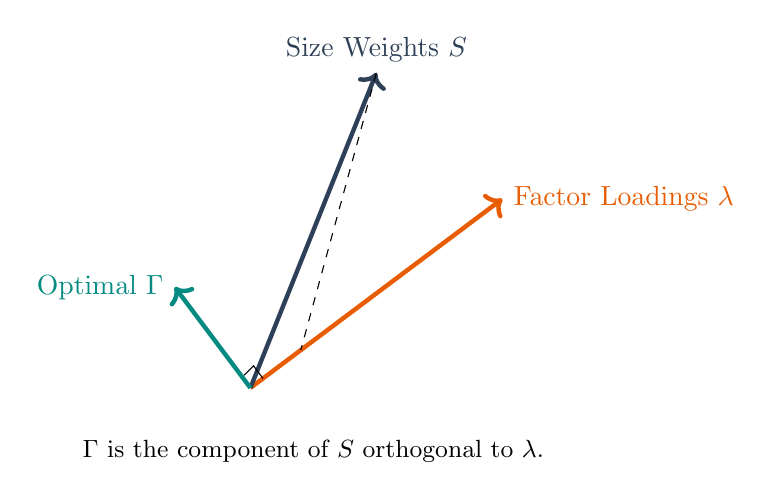
\begin{tikzpicture}[scale=0.8]
                % Vectors
                \draw[->, ultra thick, WarmOrange] (0,0) -- (4,3) node[right] {Factor Loadings $\lambda$};
                \draw[->, ultra thick, DeepNavy] (0,0) -- (2,5) node[above] {Size Weights $S$};

                % Projection
                \draw[dashed] (2,5) -- (0.8, 0.6);
                \draw[->, ultra thick, Teal] (0,0) -- (-1.2, 1.6) node[left] {Optimal $\Gamma$};

                % Right angle
                \draw (0.2,0.15) -- (0.05, 0.35) -- (-0.1, 0.2);

                \node at (1,-1) [font=\small] {$\Gamma$ is the component of $S$ orthogonal to $\lambda$.};
            \end{tikzpicture}
        \end{adjustbox}
    \end{center}
\end{frame}

%%%%%%%%%%%%%%%%%%%%%%%%%%%%%%%%%%%%%%%%%%%%%%%%%%%%%%%%%%%%%%%%%%%%%%%%%%%%%%%%
% Implementation and Assumptions
\transitionslide{Implementation and Assumptions}{Identifying wage spillovers from superstar firms}
\begin{frame}
    \frametitle{Identifying wage spillovers from superstar firms}

    \vspace{0.5cm}
    {\Large
        How do we apply GIVs to labor markets?
    }

    \vspace{1cm}
    \begin{itemize}
        \item \textbf{The granular shock:} Use idiosyncratic productivity or demand shocks of the largest employers in a region.
        \item \textbf{The instrument:} The GIV ($z_t$) aggregates these large-firm idiosyncratic shocks.
        \item \textbf{The estimation:} Instrument local or aggregate wage changes ($p_t$) using the GIV to estimate the causal impact of labor demand on wages ($\psi$).
    \end{itemize}

\end{frame}

\begin{frame}
    \frametitle{GIV precision relies on concentrated labor markets and volatile micro-shocks}

    \begin{columns}[T]
        \begin{column}{0.55\textwidth}
            \vspace{0.5cm}
            {\Large
                For the instrument to be strong, we need:
            }

            \vspace{0.8cm}
            \begin{enumerate}
                \item \textbf{A large excess Herfindahl index ($h$):} A few superstar firms must account for a substantial fraction of total employment.
                      \vspace{0.4cm}
                \item \textbf{Volatile idiosyncratic shocks ($\sigma_u$):} Firm-specific shocks must be large relative to aggregate macroeconomic volatility ($\sigma_\varepsilon$).
            \end{enumerate}
        \end{column}

        \begin{column}{0.45\textwidth}
            \vspace{1.5cm}
            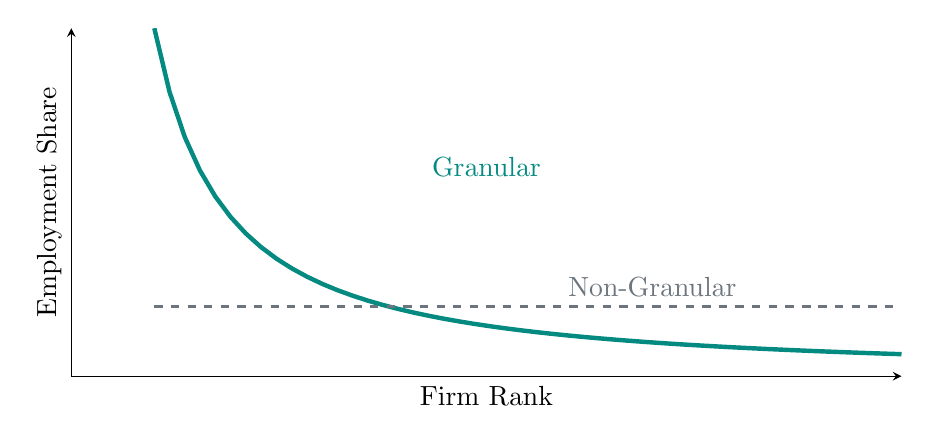
\begin{tikzpicture}
                \begin{axis}[
                        width=\textwidth, height=6cm,
                        axis lines=left,
                        xlabel={Firm Rank},
                        ylabel={Employment Share},
                        xmin=0, xmax=10,
                        ymin=0, ymax=1,
                        ticks=none
                    ]
                    \addplot[Teal, ultra thick, domain=1:10, samples=50] {1/x^1.2};
                    \node[Teal] at (axis cs: 5, 0.6) {Granular};

                    \addplot[WarmGray, thick, dashed, domain=1:10, samples=50] {0.2};
                    \node[WarmGray, anchor=south] at (axis cs: 7, 0.2) {Non-Granular};
                \end{axis}
            \end{tikzpicture}
        \end{column}
    \end{columns}

\end{frame}

\end{document}